\documentclass{article}

\usepackage[normalem]{ulem}
\usepackage{fancyhdr}
\usepackage[parfill]{parskip}
\usepackage{tikz}
\usepackage{multicol}
\usepackage{SIunits}
\pagestyle{fancyplain}
\usetikzlibrary{shapes, patterns}

\title{3.5.1 Survival and response}
\author{Todd Davies}
\date{\today}

\begin{document}

\rhead{3.5.1 Survival and response}
\lhead{\today}

\maketitle

\section*{Survival and response}
\thispagestyle{empty}

Organisms can increase their chances of survival by responding to their
enviornment. This could be by avoiding predators or moving to more hospitable
environments. They also respond to changes in their internal environemnt, for
example by increasing their metabolic rate if they become too cold. 

Any change in an (internal or external environemnt) is called a {\bf stimulus}.

\subsection*{Taxes and kineses}

There are two types of orientation movenents:

\begin{itemize}

	\item A taxis is a movement in a specific direction (usually away or towards
	a particular stimulus). Maggots have a negative phototaxis since they move
	away from light deeper into soil.

	\item A kinesis is a movement in any direction. Flatworms move in a straight
	line until they detect an increase in chemical concentration (of meat
	chemicals) in the water, which causes them to move in random circles until
	they either find the meat and begin feeding, or stop sensing the chemical
	and carry on in a straight line.

\end{itemize}

\subsection*{Reflex actions}

A reflex action is a rapid, inate, automatic response to a stimulus that
(usually) helps an organism avoid danger.

\subsection*{Tropisms}

Tropisms are responses to directional stimuli that can maintain the roots and
shoots of flowering plants in a favourable environment.

A positive tropism exhibits a tendancy towards a stimuli, while a negative
tropism exhibits a tendancy away from a stimuli.

\subsubsection*{Phototropism}

Phototropism is when plant shoots grow towards the light (and plant roots grow
away from the light). This is often why small weeds grow away from a hedge,
since they are growing towards the light that isn't taken by the hedge.

\begin{center}
	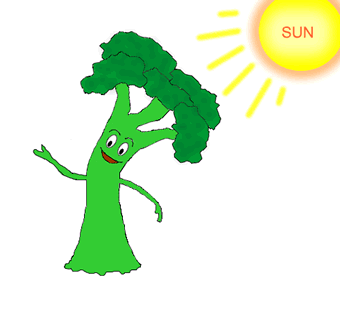
\includegraphics[scale=0.5]{phototropism}
\end{center}

\subsubsection*{Geotropism}

The shoots of plants always grow away from the direction of gravity (i.e. up),
since that is where the most light is. Roots of plants do the opposite and grow
down. If the orientation of a plant changes (e.g. an earthquake happens) then
the plant will change it's direction of growth so it is growing upwards.

\begin{center}
	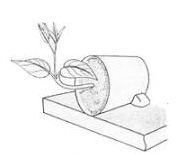
\includegraphics{geotropism}
\end{center}

\section*{Receptors}

Information from our skin allows us to identify several distinct types of
sensations, such as tapping, vibration, pressure, pain, heat and cold. Several
different types of sensory receptors respond to these different types of
stimuli.  In order to detect stimuli, the nerve endings must be adapted to
convert the mechanical, thermal or chemical energy into electrical impulses that
can travel to the brain.

\subsection*{The Pacinian corpuscle}

The Pacinian corpuscles in the skin are large for receptors, usually around 1mm
long. They consist of many concentric layers. Each layer is composed of thin,
flat cells called lamellae and fibrous connective tissue seperated by a
gelatinous material. In the center of the corpuscle, there is a fluid filled
cavity with a single axon.

\begin{center}
	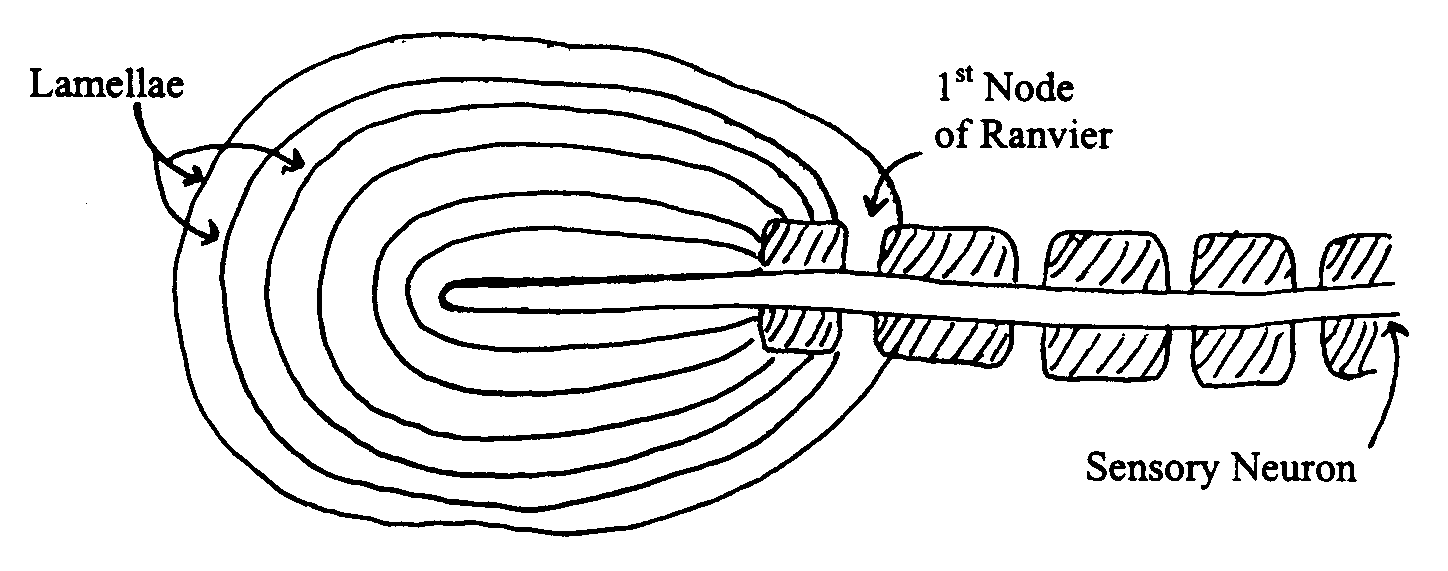
\includegraphics[scale=0.2]{pacinian_corpuscle}
\end{center}

They can only detect large pressure changes and vibrations, since these stimuli
cause compression of the capsule, resulting in deformation of the axon. Sodium
ion channels in the deformed area open, creating a generator potiential which
starts an impulse.

\subsection*{Light receptors}

There are two types of light receptors in the human retina, rods and cones. The
amount of neuroreceptor that is emmitted from a light receptor cell is
proportional to the intensity of the light.

Rod cells are specialised for dark conditions. The pigment they contain is
called rhodopsin, which makes them able to sense very small amounts of light.

Cone cells have a different pigment called iodopsin, which is only broken down
by light of high intensity.

Since the amount of neurotransmitter emmitted from rod cells is so small, there
are many of them joined to one bipolar cell (leading straight to the brain) so
that spatial summation can occur and an action potiential will be reached. This
makes rod cells very sensitive, but also means they have a low acuity.
\marginpar{\raggedright {\bf Acuity}: Sharpness or keenness of thought, vision,
or hearing.}

Cone cells almost never share a bipolar cell, and so they have a very high
acuity.

\begin{center}

	\begin{tabular}{|l|p{3.8cm}|p{3.8cm}|}

		\hline

		Property & Rods & Cones \\ \hline

		Number per eye & 120 million & 6 million\\ \hline

		Retinal convergence & 15-45 rods per bipolar cell. & 1 cone per bipolar
		cell in the fovea.\\ \hline

		Sensitivity & High - one photon gives a response. & Low - several
		hundred photons needed for a repsonse.\\ \hline

		Acuity & Poor & Good \\ \hline

	\end{tabular}

\end{center}

\begin{center}
	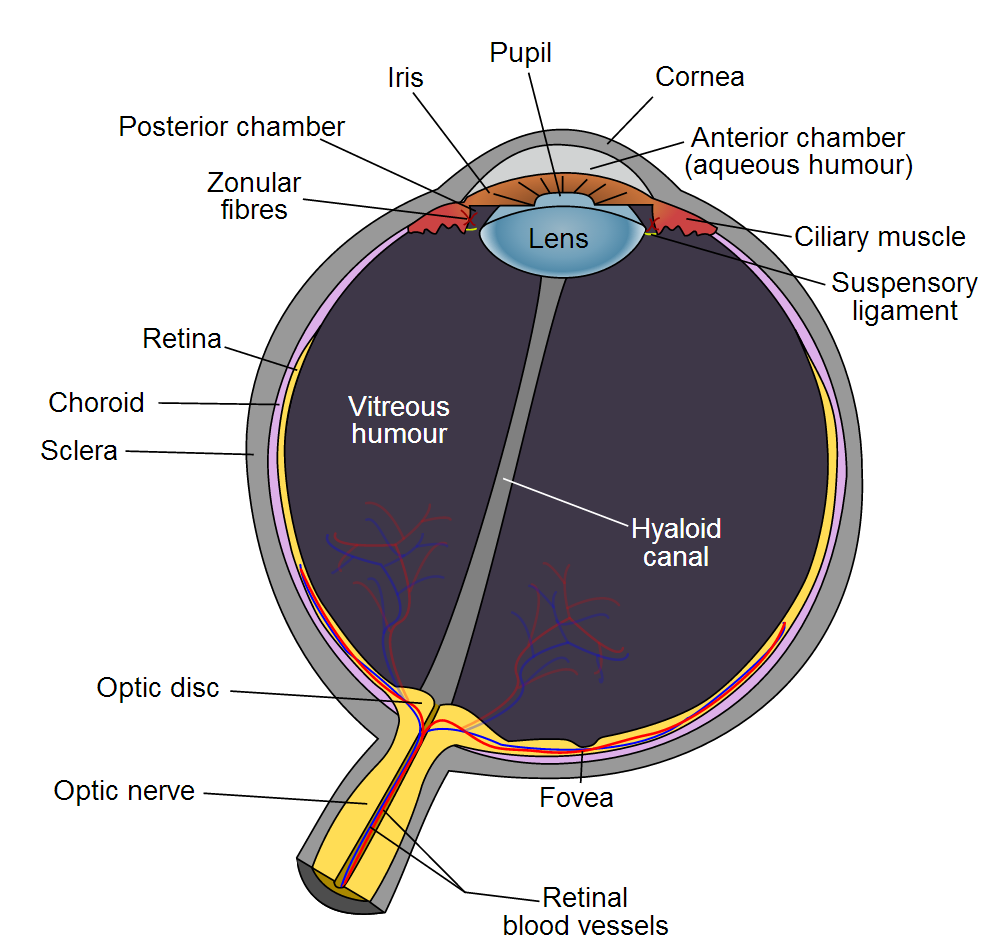
\includegraphics[scale=0.25]{eye}
\end{center}

\section*{Control of heartbeat}

The rate at which the sinoatrial node sends out impulses can be modified by the
nervous system and hormones. Modification of heartbeat is controlled by the
medulla of the brain.

Impulses via {\bf sympathetic} nerve fibres {\bf speed up} the rate at which the
sinoatrial node sends out impulses.

Impulses via {\bf parasympathetic} nerve fibres {\bf slow down} the rate at
which the sinoatrial node sends out impulses.

The medulla of the brain is influenced by pressure receptors and chemoreceptors
in the walls of the aorta and carotid sinuses. There is no direct relationship
between the oxygen and carbon dioxide concentration of the blood and the rate of
heartbeat.

\subsection*{Responses to changes in blood pressure}

When the  pressure receptors in the aorta and cartoid arteries detect a change
in pressure, one of two things happen:

\paragraph*{Increase in blood pressure} The cardioinhibitory center is
stimulated and the cardioacceleratory centre is inhibited. Impulses are sent to
a region in the medulla of the brain called the vasomotor centre. This then
sends impulses to arterioles in various part of the body, which results in
vasodilation and a drop in blood pressure.

\paragraph*{Decrease in blood pressure} The medulla sends impulses via
sympathetic nerves to the heart and arterioles. This stimulates an increase in
heart rate and vcasoconstriction in order to increase blood pressure.

\end{document}